\documentclass[11pt,a4paper]{article}
\usepackage[margin=22mm,headheight=16pt,footskip=12mm]{geometry}
\usepackage[T1]{fontenc}
\usepackage[utf8]{inputenc}
\usepackage{lmodern,amsmath,amssymb,graphicx,xcolor,booktabs,longtable,array,tabularx}
\usepackage{tikz,float,caption,fancyhdr,titlesec,url,lscape}
\usetikzlibrary{arrows.meta,positioning,calc}
\definecolor{navy}{HTML}{16324F}
\definecolor{teal}{HTML}{007F86}
\definecolor{pale}{HTML}{EAF5F5}
\definecolor{ink}{HTML}{243646}
\definecolor{amber}{HTML}{A45C13}
\pdfinfo{/Title (From Speed PI to Inverse-GPR Virtual-Fuel Control) /Author (T-MATS Controller Development Study)}
\urlstyle{tt}
\setlength{\parindent}{0pt}
\setlength{\parskip}{5pt plus 1pt minus 1pt}
\setlength{\emergencystretch}{2em}
\widowpenalty=10000\clubpenalty=10000
\linespread{1.05}
\titleformat{\section}{\Large\sffamily\bfseries\color{navy}}{\thesection}{.7em}{}
\titleformat{\subsection}{\large\sffamily\bfseries\color{teal}}{\thesubsection}{.7em}{}
\titlespacing*{\section}{0pt}{19pt}{8pt}
\titlespacing*{\subsection}{0pt}{13pt}{5pt}
\captionsetup{font=small,labelfont={bf,color=navy},skip=8pt}
\pagestyle{fancy}\fancyhf{}
\fancyhead[L]{\small\sffamily\color{navy}INVERSE-GPR VIRTUAL-FUEL PI}
\fancyhead[R]{\small\sffamily T-MATS control study}
\fancyfoot[L]{\scriptsize\color{ink}9500 rpm step tuning / fixed-controller comparison}
\fancyfoot[R]{\small\thepage}
\renewcommand{\headrulewidth}{.3pt}
\tikzset{block/.style={draw=navy!55,fill=navy!3,rounded corners=3pt,minimum height=.92cm,align=center,font=\sffamily\small,inner sep=5pt},
gp/.style={block,draw=teal,fill=pale},plant/.style={block,draw=navy,fill=navy!12},
sum/.style={circle,draw=navy,minimum size=.68cm,fill=white,font=\large},
arr/.style={-{Latex[length=2.2mm]},draw=navy,line width=.65pt},
lab/.style={font=\small,fill=white,inner sep=2pt},
note/.style={font=\small\sffamily,text=ink,align=left}}
\begin{document}
\begin{titlepage}
\color{navy}\sffamily
{\small T-MATS / CONTROLLER DEVELOPMENT TUTORIAL}\par\vspace{18mm}
{\fontsize{30}{36}\selectfont\bfseries From Speed PI to\\Inverse-GPR\\Virtual-Fuel Control\par}
\vspace{9mm}{\Large Ideation, derivation, uncertainty experiments,\\and fixed-gain retuning for reduced fuel ringing\par}
\vspace{10mm}\color{teal}\rule{\linewidth}{1.2pt}\color{navy}\vspace{8mm}
\begin{tabular}{@{}ll}
Selected fuel-domain gains & $K_p=2,\ K_i=30\ \mathrm{s}^{-1}$\\[5pt]
Tuning condition & 9500 rpm, 5\% shaft-load steps\\[5pt]
Final comparison & Four controllers, eleven cases, 44 fresh runs\\[5pt]
Sample interval & 0.015 s\\[5pt]
Report date & 14 September 2026
\end{tabular}
\par\vspace{12mm}\normalfont\color{ink}
\textbf{Measured tuning outcome.} Lowering the fuel-domain gains from (3,60) to (2,30) reduced ringing by 90.4\% on the 9500 rpm, 5\% step tuning case. Speed RMSE changed from 0.712 to 0.930 rpm (30.7\% higher). This is a measured damping-versus-tracking tradeoff.

This tutorial derives the controllers, explains derivative-like feedback and fuel ringing, and compares speed accuracy, fuel oscillation, recovery and physical validity. The uncertainty schedules are earlier design hypotheses; the final comparison uses fixed gains.

\vfill Numerical simulations under the specified T-MATS configuration. Invalid trajectories receive no full-run performance scores. MATLAB sources, raw trajectories, tables and LaTeX source accompany this report.
\end{titlepage}
\tableofcontents\clearpage
\section{Ideation: from shaft-speed error to virtual fuel}
A shaft-load disturbance extracts additional power. The shaft initially decelerates, and the controller must add fuel to recover speed. Removing the load requires the opposite adjustment. Fast recovery and smooth fuel motion compete: rotor inertia can hide rapid fuel oscillations behind a comparatively smooth speed trace.

The investigation began with the inherited speed PI, then learned an inverse Gaussian-process regression mapping from shaft motion to nominal fuel. The same GP evaluated desired and measured motion, and their difference drove a fuel-domain PI. GPR feedforward and two uncertainty gain schedules were subsequently tested. The final step returned to fixed lower gains and explicitly constrained ringing rather than minimizing speed RMSE alone.

The earlier inverse-GPR PI used $(4,40)$, selected on 9000 rpm ramps. The later fixed FF pair $(3,60)$ and uncertainty schedules are historical comparison stages. The final pair $(2,30)$ is selected on 9500 rpm, 5\% steps and frozen for the eleven-case rerun.

\subsection{Physical disturbance path}
In consistent SI units, a simplified shaft balance is
\begin{equation}
J\dot\omega=\tau_t-\tau_c-\tau_L,\qquad N=\frac{60}{2\pi}\omega,\qquad \tau_L=P_L/\omega.
\label{eq:shaft}
\end{equation}
The simulation retains the existing T-MATS component maps and iterative thermodynamic solver. T-MATS is NASA's thermodynamic-system modeling toolbox~\cite{tmats}; the plant is not replaced by a GP. Equation~\eqref{eq:shaft} explains the mechanism rather than replacing the implementation's horsepower and rpm conversions. Load percentage refers to nominal turbine power at the case speed, not fuel flow. Neither the future load schedule nor the injected shaft-load signal enters any controller.

\begin{table}[H]\centering\small
\begin{tabularx}{\linewidth}{@{}lXl@{}}\toprule Symbol & Meaning & Unit\\\midrule
$r,N,N_s$ & Governed reference, actual speed, sensed speed & rpm\\
$a_r,\hat a_s$ & Reference acceleration, estimated sensed acceleration & rpm/s\\
$g(N,a)$ & Frozen inverse-GPR mean fuel & lbm/s\\
$v_r,v_y,e_v$ & Virtual setpoint, virtual feedback and their difference & lbm/s\\
$I,u^\star,u$ & Integral, unsaturated and limited command & lbm/s\\
$\sigma_r,\sigma_y$ & Response SD of the two GP queries & lbm/s\\
$K_p,K_i$ & Fuel-domain PI gains & 1, s$^{-1}$\\\bottomrule
\end{tabularx}\caption{PI gain units depend on the error coordinate.}\end{table}

\section{Learning and interpreting the inverse GP}
The nominal inverse estimates
\begin{equation}w=g(N,a),\qquad x=[N\quad a]^{\mathsf T}.\end{equation}
It is fitted directly to speed, plant acceleration and fuel samples, not obtained by algebraically inverting a forward GP. The archived exact GP uses 600 training points and 100 held-out points in the 9000--10000 rpm region at fixed ambient conditions and zero external shaft load. Its test fuel RMSE is 0.0010482 lbm/s; empirical coverage of the nominal 95\% response interval is 97\%. These are prediction results, not closed-loop guarantees.

For standardized inputs and targets, the kernel and exact posterior are~\cite{gpml}
\begin{align}
k(z,z')&=\sigma_f^2\exp\left[-\frac12\sum_{d=1}^2(z_d-z'_d)^2/\ell_d^2\right],\\
K_y&=K+\sigma_n^2I=LL^{\mathsf T},\quad
\boldsymbol\alpha=L^{-\mathsf T}L^{-1}\widetilde{\boldsymbol w},\\
g(x_*)&=\mu_w+s_w\boldsymbol k_*^{\mathsf T}\boldsymbol\alpha,\\
\sigma_{\rm response}^2(x_*)&=s_w^2\left[\max(0,k_{**}-\|L^{-1}\boldsymbol k_*\|^2)+\sigma_n^2\right].
\label{eq:gpvar}
\end{align}
Latent variance omits the noise term; scheduling used response SD. The posterior remains frozen throughout all controller trials. Comparison cases do not retrain it.
\begin{figure}[H]\centering\resizebox{\linewidth}{!}{
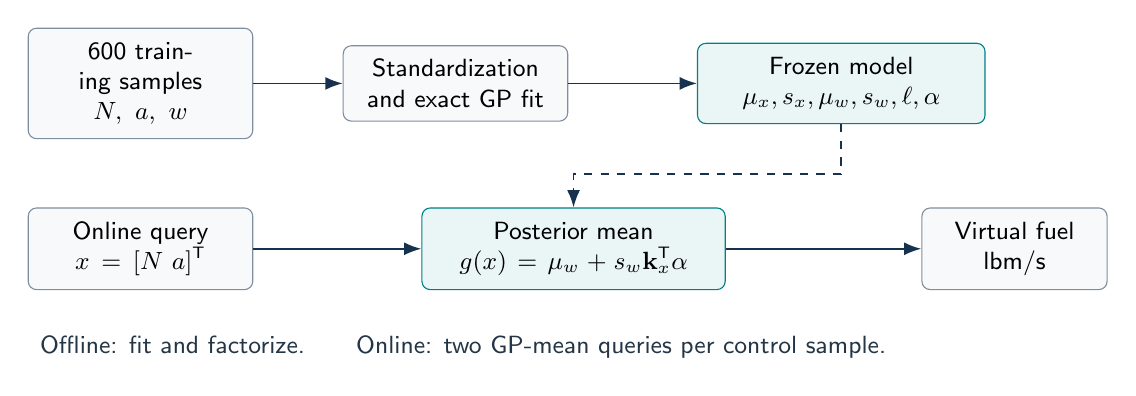
\begin{tikzpicture}[x=1cm,y=1cm]
\node[block,text width=2.5cm] (data) at (1.4,0) {600 training samples\\$N,\ a,\ w$};
\node[block,text width=2.5cm] (fit) at (5.4,0) {Standardization\\and exact GP fit};
\node[gp,text width=3.3cm] (model) at (10.3,0) {Frozen model\\$\mu_x,s_x,\mu_w,s_w,\ell,\alpha$};
\draw[arr](data)--(fit);\draw[arr](fit)--(model);
\node[block,text width=2.5cm] (query) at (1.4,-2.1) {Online query\\$x=[N\ a]^{\mathsf T}$};
\node[gp,text width=3.5cm] (pred) at (6.9,-2.1) {Posterior mean\\$g(x)=\mu_w+s_w\mathbf{k}_x^{\mathsf T}\alpha$};
\node[block,text width=2cm] (out) at (12.5,-2.1) {Virtual fuel\\lbm/s};
\draw[arr](query)--(pred);\draw[arr](pred)--(out);
\draw[arr,dashed](model.south)--(10.3,-1.15)-|(pred.north);
\node[note,anchor=west] at (0,-3.35) {Offline: fit and factorize.\qquad Online: two GP-mean queries per control sample.};
\end{tikzpicture}
}\caption{Frozen inverse-GPR training and online mean evaluation. The saved Cholesky factor supplies uncertainty when scheduling is active.}\end{figure}

\subsection{Nominal coordinates are not an external-load estimate}
Desired and measured motion are mapped into nominal fuel units. Under load, the GP output need not equal the actual fuel required. The integral supplies residual fuel to balance the load. Thus the controller can use a nominal inverse without claiming that it has learned that disturbance.

Predictive SD is conditional on the fitted model. It does not automatically quantify unknown shaft load, ambient variation, sensor-input uncertainty or hyperparameter uncertainty. A confident GP and an inadequate loaded-plant controller can coexist. Speed excursions below 9000 rpm are logged as leaving the virtual-fuel model's training range rather than concealed by input clipping.

\section{Derivation of the four fixed architectures}
\subsection{Base speed PI}
For $e_N=r-N_s$, the original controller has the conceptual PI form
\begin{equation}
u_b^\star=K_{p,N}e_N+I_b,\quad \dot I_b=K_{i,N}e_N,\quad K_{p,N}=0.025,\quad K_{i,N}=0.05.
\end{equation}
The existing library PI and its initialization remain unchanged. Its gains act on rpm error and are not numerically comparable to fuel-domain gains. All final methods share the downstream fuel limits.

\subsection{Base PI plus the existing GPR correction}
For continuity with the preceding study, this method retains the state-scheduled nominal correction
\begin{align}
a_r[k]&=\operatorname{clip}((r[k]-r[k-1])/T_s,-150,150),\\
N_q[k]&=\operatorname{clip}(N_s[k],9000,10000),\\
b[k]&=\rho[k]\operatorname{clip}(g(N_q[k],a_r[k])-g(N_0,0),-0.15,0.15),\\
u[k]&=\operatorname{sat}(u_b[k]+b[k]),\quad \rho(t)=\operatorname{clip}((t-30)/2,0,1).
\label{eq:baseff}
\end{align}
Equilibrium subtraction avoids adding nominal fuel twice, since the original PI integral already supplies it. Sensed speed enters this GP, so it is not reference-only feedforward. At constant reference, $a_r=0$, but $b$ may still change with sensed speed.

\subsection{Inverse-GPR virtual-fuel PI}
The two inverse evaluations define
\begin{equation}
v_r=g(r,a_r),\qquad v_y=g(N_s,\hat a_s),\qquad e_v=v_r-v_y.
\label{eq:virtual}
\end{equation}
The discrete PI forms
\begin{equation}
u^\star[k]=K_pe_v[k]+I[k],\qquad I[k+1]=I[k]+T_sK_ie_v[k]
\label{eq:invpi}
\end{equation}
when integration is permitted. Feedback is virtual fuel inferred from motion, not actual measured fuel. The error contains acceleration as well as speed.
\begin{figure}[H]\centering\resizebox{\linewidth}{!}{
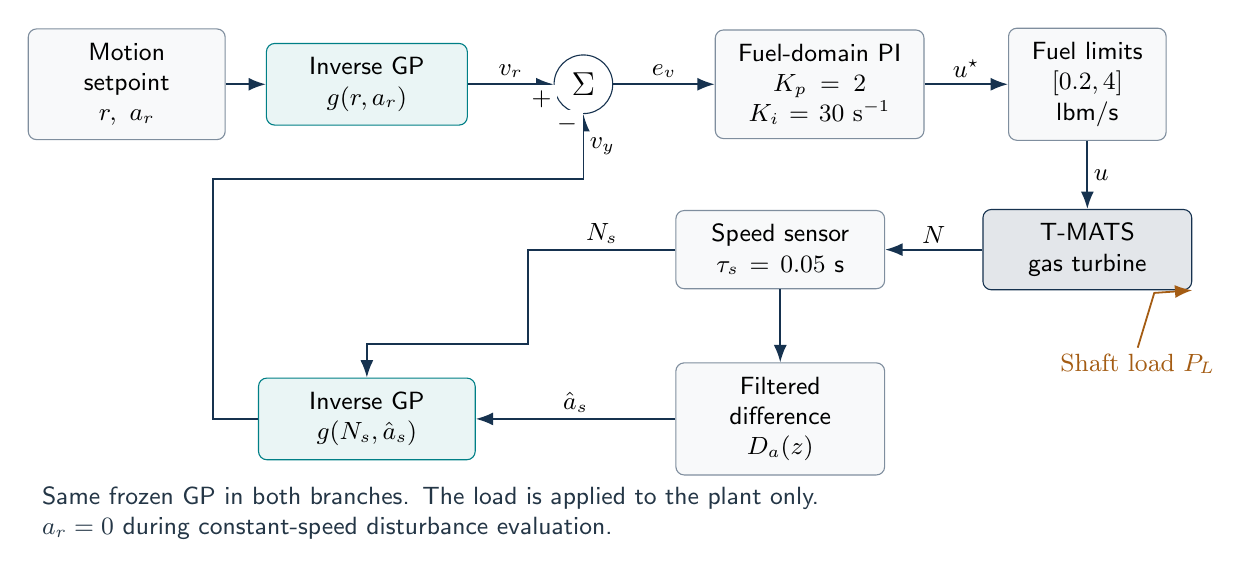
\begin{tikzpicture}[x=1cm,y=1cm]
\node[block, text width=2.15cm] (ref) at (1.2,0) {Motion setpoint\\$r,\ a_r$};
\node[gp, text width=2.2cm] (gr) at (4.25,0) {Inverse GP\\$g(r,a_r)$};
\node[sum] (err) at (7,0) {$\Sigma$};
\node[block,text width=2.3cm] (pi) at (10,0) {Fuel-domain PI\\$K_p=2$\\$K_i=30\ \mathrm{s}^{-1}$};
\node[block,text width=1.65cm] (lim) at (13.4,0) {Fuel limits\\$[0.2,4]$\\lbm/s};
\node[plant,text width=2.3cm] (engine) at (13.4,-2.1) {T-MATS\\gas turbine};
\node[block,text width=2.3cm] (sensor) at (9.5,-2.1) {Speed sensor\\$\tau_s=0.05$ s};
\node[gp,text width=2.4cm] (gy) at (4.25,-4.25) {Inverse GP\\$g(N_s,\hat a_s)$};
\node[block,text width=2.3cm] (diff) at (9.5,-4.25) {Filtered difference\\$D_a(z)$};
\draw[arr] (ref)--(gr);
\draw[arr] (gr)--node[above,lab]{$v_r$}node[pos=.86,below,lab]{$+$}(err);
\draw[arr] (err)--node[above,lab]{$e_v$}(pi);
\draw[arr] (pi)--node[above,lab]{$u^\star$}(lim);
\draw[arr] (lim)--node[right,lab]{$u$}(engine);
\draw[arr] (engine)--node[above,lab]{$N$}(sensor);
\draw[arr] (sensor.west)--node[above,lab]{$N_s$}(6.3,-2.1)--(6.3,-3.3)--(4.25,-3.3)--(gy.north);
\draw[arr] (sensor)--(diff);
\draw[arr] (diff)--node[above,lab]{$\hat a_s$}(gy);
\draw[arr] (gy.west)--(2.3,-4.25)--(2.3,-1.2)--(7,-1.2)--node[right,lab]{$v_y$}node[pos=.85,left,lab]{$-$}(err.south);
\node[lab,anchor=east,text=amber] (load) at (15.1,-3.55) {Shaft load $P_L$};
\draw[arr,draw=amber] (load.north)--(14.25,-2.65)--(engine.south east);
\node[note,anchor=west,text width=11cm] at (0,-5.45) {Same frozen GP in both branches. The load is applied to the plant only.\\$a_r=0$ during constant-speed disturbance evaluation.};
\end{tikzpicture}
}\caption{Virtual-fuel feedback. The FF extension adds the virtual reference fuel before the common limits.}\end{figure}

\subsection{Inverse-GPR PI plus reference fuel feedforward}
The nominal setpoint fuel is added directly:
\begin{equation}
u^\star[k]=v_r[k]+K_pe_v[k]+I_{\rm res}[k],\qquad
I_{\rm res}[k+1]=I_{\rm res}[k]+T_sK_ie_v[k].
\label{eq:invff}
\end{equation}
The integral supplies the residual beyond nominal feedforward. Both inverse variants in the final comparison use $K_p=2$, $K_i=30$ s$^{-1}$, the same frozen GP, sensing, sample timing and limits.

\subsection{Constant-reference equivalence}
The reference has settled before handover, so $v_r=c$ is constant. Initializing
\begin{equation}I_{\rm noFF}[k_0]=c+I_{\rm res}[k_0]\end{equation}
and applying identical integral increments preserves the offset:
\begin{equation}
I_{\rm noFF}[k]=c+I_{\rm res}[k]\quad\Longrightarrow\quad
u^\star_{\rm noFF}[k]=u^\star_{\rm FF}[k].
\label{eq:equivalence}
\end{equation}
Identical saturation and anti-windup decisions then preserve matching trajectories, apart from numerical effects. This requires constant $v_r$ and matched states. Changing-reference behavior is a different experiment. Overlap of the inverse-GPR pair is expected here and does not prove that feedforward lacks a reference-tracking benefit.

\section{Why virtual-fuel PI can produce fuel ringing}
Let $c_N=\partial g/\partial N$ and $c_a=\partial g/\partial a$ at $(N_0,0)$. Linearization gives
\begin{equation}e_v\simeq c_N(r-N_s)+c_a(a_r-\hat a_s).\end{equation}
With constant reference and ideal acceleration, $\hat a_s=-\dot e_N$, giving
\begin{align}
\frac{\delta u(s)}{e_N(s)}
&\simeq\left(K_p+\frac{K_i}{s}\right)(c_N+c_as)\\
&=K_pc_as+(K_pc_N+K_ic_a)+\frac{K_ic_N}{s}.
\label{eq:localpid}
\end{align}
The outer PI therefore contains derivative-like action through the inverse acceleration input. Increasing $K_p$ amplifies this path, while $K_i$ contributes to the local proportional term. This is a local zero-state interpretation, not a nonlinear sampled-system stability proof.
\begin{figure}[H]\centering\resizebox{\linewidth}{!}{
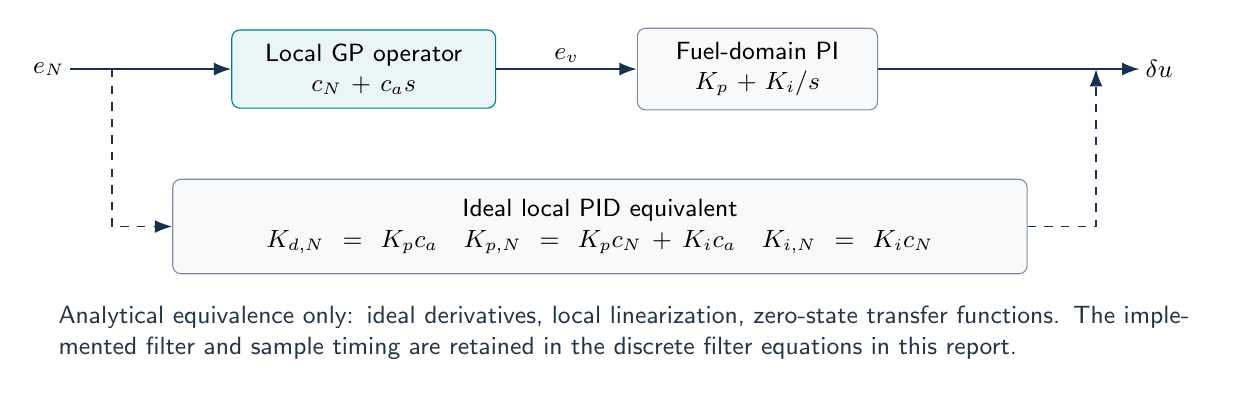
\begin{tikzpicture}[x=1cm,y=1cm]
\node[lab] (e) at (0,0) {$e_N$};
\node[gp,text width=3cm] (g) at (4,0) {Local GP operator\\$c_N+c_as$};
\node[block,text width=2.7cm] (pi) at (9,0) {Fuel-domain PI\\$K_p+K_i/s$};
\node[lab] (u) at (14.1,0) {$\delta u$};
\draw[arr](e)--(g);\draw[arr](g)--node[above,lab]{$e_v$}(pi);\draw[arr](pi)--(u);
\node[block,text width=10.5cm,minimum height=1.2cm] (equiv) at (7,-2) {Ideal local PID equivalent\\$K_{d,N}=K_pc_a\quad K_{p,N}=K_pc_N+K_ic_a\quad K_{i,N}=K_ic_N$};
\draw[arr,dashed](.8,0)|-(equiv.west);\draw[arr,dashed](equiv.east)-|(13.3,0);
\node[note,anchor=west,text width=14.6cm] at (0,-3.35) {Analytical equivalence only: ideal derivatives, local linearization, zero-state transfer functions. The implemented filter and sample timing are retained in the discrete filter equations in this report.};
\end{tikzpicture}
}\caption{Local ideal PID interpretation of fuel-coordinate PI. The implemented acceleration filter and sample timing remain essential.}\end{figure}

Rotor inertia can attenuate rapid fuel variations while speed RMSE remains small. Tuning only that RMSE can favor an oscillatory fuel command. Lowering gains changes derivative-like, proportional and integral behavior together. This motivates a separate ringing metric and an explicit ringing constraint.

\section{Causality, handover and anti-windup}
The inherited speed sensor has a 0.05 s time constant; optional sensor-noise injection is disabled. Acceleration is estimated causally:
\begin{align}
p_a&=\exp(-T_s/0.03),\\
\hat a_s[k]&=p_a\hat a_s[k-1]+(1-p_a)(N_s[k]-N_s[k-1])/T_s,\\
D_a(z)&=\frac{(1-p_a)(1-z^{-1})}{T_s(1-p_az^{-1})},\quad T_s=0.015\ {\rm s}.
\end{align}
Filtering limits differentiation but does not remove its fast feedback path.

Before handover at 30 s, integral tracking uses $I=u_b-K_pe_v$ without FF and $I_{\rm res}=u_b-v_r-K_pe_v$ with FF. This avoids double counting fuel and supplies the offset in Equation~\eqref{eq:equivalence}. The common limits and integration rule are
\begin{align}
u&=\max(0.2,\min(4,u^\star)),\\
\text{integrate if}\quad&
(u^\star<4\ \text{or}\ e_v<0)\ \text{and}\
(u^\star>0.2\ \text{or}\ e_v>0).
\end{align}
Errors may unwind saturation but cannot wind the integral farther into it. The test applies to the entire FF-plus-PI command.

\section{Uncertainty scheduling: two hypotheses}
The earlier schedules used
\begin{equation}
q=\frac{\max(\sigma_r,\sigma_y)}{\sigma_0},\qquad \sigma_0=0.00117869140424\ {\rm lbm/s},
\end{equation}
with the reference equal to median response SD at the 600 training inputs. The decreasing rule was
\begin{equation}\gamma_\downarrow(q)=10^{-(q/3)^2}.\end{equation}
Both gains fall to 10\% at $q=3$ and approach zero. The increasing alternative was
\begin{equation}
x=\operatorname{clip}((q-1)/2,0,1),\qquad \gamma_\uparrow=1+3x^2-2x^3.
\end{equation}
It equals 1 up to one reference SD, 1.5 at two, and 2 at three and beyond, with zero endpoint slopes. SD is nonnegative; the plus/minus bands refer to magnitude, not control-error sign.

Both schedules multiply $K_p$ and $K_i$. Gain changes transfer $(K_{p,\rm old}-K_{p,\rm new})e_v$ into the integral to avoid a command jump due solely to scheduling. Accumulated load compensation remains even when further integral increments shrink.

Archived ten-case studies passed 9 cases for the earlier inverse-GPR PI at $(4,40)$, 7 for fixed FF at $(3,60)$, 8 for decreasing gains, and 7 for increasing gains. Increasing gains produced about 2.0--2.8 times the decreasing schedule's ringing on seven mutually valid ramp cases. Decreasing gains restored the 9500 rpm, 20\% step case and raised minimum surge margin to 4.96\%, but increased RMSE to 3.76 rpm versus 3.10 rpm for the older $(4,40)$ controller.

These findings motivated fixed-gain retuning. GP confidence and feedback damping requirements are different quantities under unmodeled loads. Neither scheduling direction is universally preferred. No uncertainty schedule is active in the final four-controller reruns.

\section{Test protocol and performance definitions}
Each run has 60 s preparation and 90 s evaluation, with 10,001 samples over 150 s. The demand transitions from 10,000 rpm to the case speed before evaluation. Load pulses start at evaluation times 10.005, 30 and 60 s and end at 15, 40.005 and 75 s. Ramp durations are 0.3, 1.5 and 3 s; steps use zero duration.
\begin{table}[H]\centering\small
\begin{tabular}{@{}lrll@{}}\toprule
Case & Speed [rpm] & Load & Shape\\\midrule
C1 & 9000 & 5\% & ramps\\
C2 & 9000 & 10\% & ramps\\
C3 & 9000 & 20\% & ramps\\
C4 & 9000 & 30\% & ramps\\
C5 & 9500 & 5\% & ramps\\
C6 & 9500 & 10\% & ramps\\
C7 & 9500 & 20\% & ramps\\
C8 & 9500 & 30\% & ramps\\
C9 & 9500 & 20\% & steps\\
C10 & 9500 & 30\% & steps\\
C11 & 9500 & 5\% & steps\\
\bottomrule\end{tabular}\caption{The eleven final comparison cases. C11 is the tuning condition.}\end{table}


\subsection{Speed RMSE and fuel ringing}
For evaluation errors $e_i=N_i-r$,
\begin{equation}
{\rm RMSE}_N=\sqrt{\frac1n\sum_i e_i^2},\qquad {\rm IAE}_N=T_s\sum_i|e_i|.
\end{equation}
For each of six load transitions, consider the two seconds after its ramp finishes or immediately after its step. With window fuel samples $w_1,\ldots,w_m$, define
\begin{equation}
R_j=\max\left(0,\sum_{i=2}^m|w_i-w_{i-1}|-|w_m-w_1|\right),\qquad R=\sum_{j=1}^6R_j.
\label{eq:ring}
\end{equation}
This excess total variation measures repeated reversals beyond net monotonic adjustment. Units are lbm/s. It is not a single oscillation amplitude, fuel consumption or a direct actuator-wear measure. Maximum two-second peak-to-peak fuel range and sampled slew are logged separately. All comparisons use the same windows and sample interval.

\subsection{Recovery to a 1\% speed window}
Recovery is measured from each transition onset to the first sample after which speed remains inside the band until the next transition:
\begin{equation}
T_{1\%,j}=\inf\{\tau\geq0:\ |N(t)-r|\leq0.01r
\text{ at all remaining samples in the event interval}\}.
\end{equation}
The tables report the maximum across six events. If a response never leaves the band, recovery is zero; if it never settles before the next event, it is unrecovered. The band is $\pm90$ rpm at 9000 rpm and $\pm95$ rpm at 9500 rpm, not 1\% of a transient peak. A stricter $\pm0.1$ rpm measure is included because small-load responses may remain inside the 1\% band throughout.

\subsection{Validity and withheld scores}
All logged signals must remain finite, fuel positive, maximum flow residual at most $10^{-9}$, solver iterations below 200, and surge margin positive. Pre-disturbance speed error must be below 0.1 rpm. The runners check sample counts, load replay, GP predictions and command composition. A failed full-trajectory test withholds full-run RMSE, ringing and recovery scores. Plots stop at the first invalid sample; disappearing traces do not indicate recovery.

\section{Fixed-gain tuning at 9500 rpm and 5\% steps}
The criterion was fixed before selecting the result: require at least 90\% ringing reduction relative to $(3,60)$, then choose the lowest speed RMSE among valid candidates meeting that constraint. This is a finite local search, not a global optimum.
\begin{table}[H]\centering\small
\begin{tabular}{@{}lrrrrrr@{}}\toprule
ID & $K_p$ & $K_i$ & RMSE & Ringing & Reduction [\%] & $T_{0.1}$\\\midrule
1 & 3 & 60 & 0.712 & 25.8 & 0 & 3.53\\
2 & 3 & 40 & 0.721 & 6.65 & 74.2 & 2.94\\
3 & 2.5 & 40 & 0.736 & 5.08 & 80.3 & 2.92\\
4 & 2 & 40 & 0.765 & 4.84 & 81.2 & 2.91\\
5* & 2 & 30 & 0.93 & 2.49 & 90.4 & 3.17\\
6 & 1.5 & 30 & 0.967 & 2.5 & 90.3 & 3.15\\
7 & 1.5 & 20 & 1.34 & 0.959 & 96.3 & 3.53\\
8 & 1 & 20 & 1.39 & 1.11 & 95.7 & 3.5\\
9 & 1 & 10 & 2.52 & 0.0266 & 99.9 & 4.17\\
10 & 0.5 & 10 & 2.64 & 0.194 & 99.2 & 4.11\\
11 & 0.5 & 5 & 4.78 & 0.00351 & 100 & 4.91\\
12 & 0.25 & 5 & 4.96 & 0.0104 & 100 & 4.83\\
\bottomrule\end{tabular}\caption{Twelve fixed-gain candidates on 9500 rpm, 5\% steps. RMSE is in rpm; ringing in lbm/s; recovery in seconds. The asterisk marks the selected pair.}\end{table}

Lowering the fuel-domain gains from (3,60) to (2,30) reduced ringing by 90.4\% on the 9500 rpm, 5\% step tuning case. Speed RMSE changed from 0.712 to 0.930 rpm (30.7\% higher). This is a measured damping-versus-tracking tradeoff. The allowable ringing threshold was 2.5782 lbm/s; the selected result was 2.4878 lbm/s. The worst recovery to 0.1 rpm changed from 3.525 to 3.165 s. No further gains were adjusted on the transfer cases.
\begin{figure}[H]\centering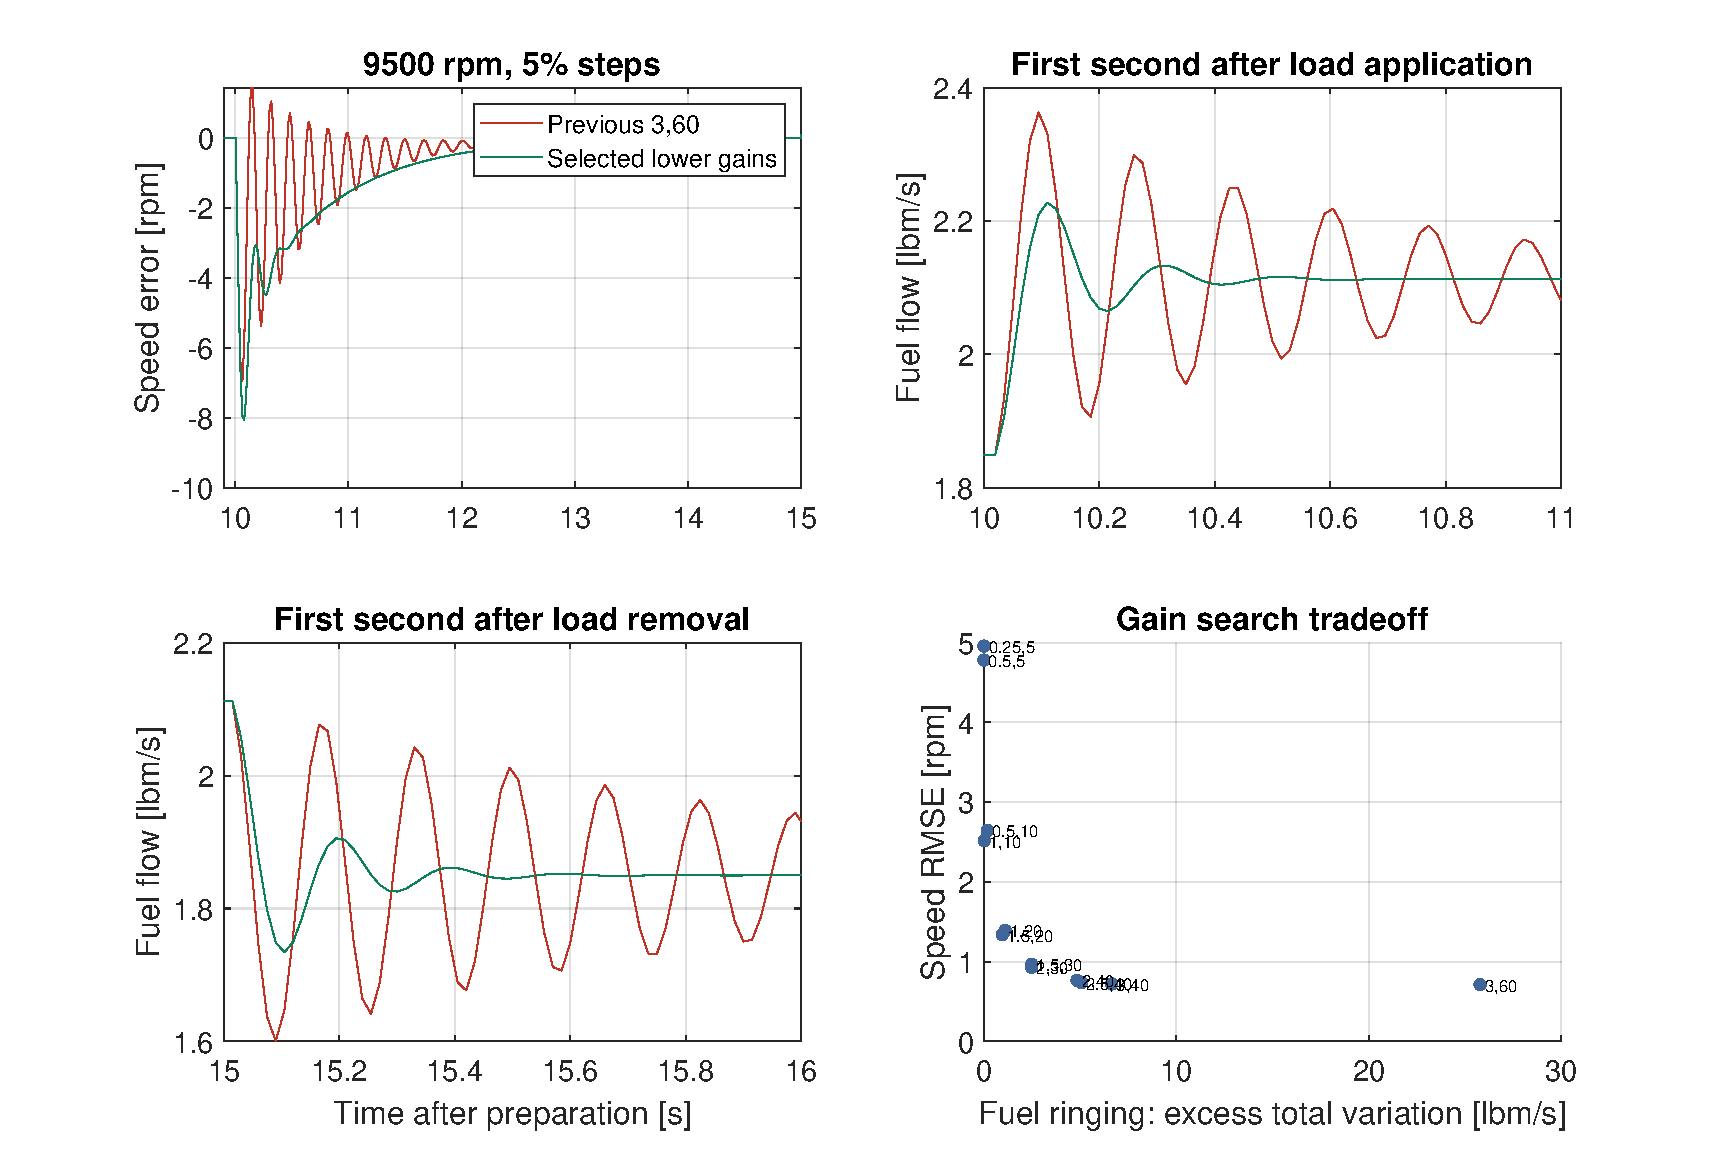
\includegraphics[width=\linewidth]{tuning_tradeoff.pdf}
\caption{Tuning-condition load and unload detail, and the fixed-gain tradeoff. Scatter labels are $(K_p,K_i)$. Lower ringing and lower speed RMSE compete.}\end{figure}

\clearpage\section{Fresh four-controller comparison}
Base speed PI retains $(0.025,0.05)$. Both inverse-GPR variants use $(2,30)$, isolating their feedforward difference from gain changes. Base PI FF remains state-scheduled as in Equation~\eqref{eq:baseff}; inverse-GPR FF remains reference-based as in Equation~\eqref{eq:invff}.
Valid runs out of eleven: P=9, PF=9, V=9, VF=9. 8 invalid runs have their full-run performance metrics withheld. All four methods were rerun after the gain selection; archived trajectories were not substituted for these runs. Invalid conditions are listed in the supplementary failure table and identified by dashes below.
\begin{table}[H]\centering\small
\begin{tabular}{@{}lrrrr@{}}\toprule
rpm/load/type & P & PF & V & VF\\\midrule
9000/5\%/R & 0.594 & 0.601 & 0.499 & 0.499\\
9000/10\%/R & 1.19 & 1.21 & 1 & 1\\
9000/20\%/R & 2.54 & 2.57 & 2.13 & 2.13\\
9000/30\%/R & 3.97 & 4.02 & 3.33 & 3.33\\
9500/5\%/R & 1.02 & 1.05 & 0.703 & 0.703\\
9500/10\%/R & 2.13 & 2.19 & 1.47 & 1.47\\
9500/20\%/R & 4.45 & 4.59 & 3.08 & 3.08\\
9500/30\%/R & -- & -- & -- & --\\
9500/20\%/S & 6.43 & 6.71 & 4.05 & 4.05\\
9500/30\%/S & -- & -- & -- & --\\
9500/5\%/S & 1.48 & 1.55 & 0.93 & 0.93\\
\bottomrule\end{tabular}\caption{Full-run speed RMSE [rpm]. P: base PI; PF: base PI plus GPR FF; V: inverse-GPR PI; VF: inverse-GPR PI plus FF. R: ramps; S: steps. A dash denotes an invalid full run; NR denotes no recovery before the next event.}\end{table}

\begin{table}[H]\centering\small
\begin{tabular}{@{}lrrrr@{}}\toprule
rpm/load/type & P & PF & V & VF\\\midrule
9000/5\%/R & 0.138 & 0.14 & 0.101 & 0.101\\
9000/10\%/R & 0.276 & 0.279 & 0.2 & 0.2\\
9000/20\%/R & 0.59 & 0.599 & 0.393 & 0.393\\
9000/30\%/R & 0.946 & 0.957 & 0.552 & 0.552\\
9500/5\%/R & 0.198 & 0.206 & 0.158 & 0.158\\
9500/10\%/R & 0.417 & 0.434 & 0.319 & 0.319\\
9500/20\%/R & 0.892 & 0.926 & 0.629 & 0.629\\
9500/30\%/R & -- & -- & -- & --\\
9500/20\%/S & 4.71 & 4.31 & 9.17 & 9.17\\
9500/30\%/S & -- & -- & -- & --\\
9500/5\%/S & 1.19 & 1.09 & 2.49 & 2.49\\
\bottomrule\end{tabular}\caption{Six-window fuel-ringing excess total variation [lbm/s]. P: base PI; PF: base PI plus GPR FF; V: inverse-GPR PI; VF: inverse-GPR PI plus FF. R: ramps; S: steps. A dash denotes an invalid full run; NR denotes no recovery before the next event.}\end{table}

\clearpage
\begin{table}[H]\centering\small
\begin{tabular}{@{}lrrrr@{}}\toprule
rpm/load/type & P & PF & V & VF\\\midrule
9000/5\%/R & 0 & 0 & 0 & 0\\
9000/10\%/R & 0 & 0 & 0 & 0\\
9000/20\%/R & 0 & 0 & 0 & 0\\
9000/30\%/R & 0 & 0 & 0 & 0\\
9500/5\%/R & 0 & 0 & 0 & 0\\
9500/10\%/R & 0 & 0 & 0 & 0\\
9500/20\%/R & 0 & 0 & 0 & 0\\
9500/30\%/R & -- & -- & -- & --\\
9500/20\%/S & 0 & 0 & 0 & 0\\
9500/30\%/S & -- & -- & -- & --\\
9500/5\%/S & 0 & 0 & 0 & 0\\
\bottomrule\end{tabular}\caption{Worst recovery to a 1\% commanded-speed band [s], measured from transition onset. P: base PI; PF: base PI plus GPR FF; V: inverse-GPR PI; VF: inverse-GPR PI plus FF. R: ramps; S: steps. A dash denotes an invalid full run; NR denotes no recovery before the next event.}\end{table}

\begin{table}[H]\centering\small
\begin{tabular}{@{}lrrrr@{}}\toprule
rpm/load/type & P & PF & V & VF\\\midrule
9000/5\%/R & 4.09 & 4.08 & 5.06 & 5.06\\
9000/10\%/R & 4.44 & 4.39 & 5.67 & 5.67\\
9000/20\%/R & 4.77 & 4.75 & 6.33 & 6.33\\
9000/30\%/R & 4.96 & 4.93 & 6.71 & 6.71\\
9500/5\%/R & 4.38 & 4.26 & 5.1 & 5.1\\
9500/10\%/R & 4.72 & 4.56 & 5.7 & 5.7\\
9500/20\%/R & 5.06 & 4.88 & 6.29 & 6.29\\
9500/30\%/R & -- & -- & -- & --\\
9500/20\%/S & 2.98 & 2.75 & 4.34 & 4.34\\
9500/30\%/S & -- & -- & -- & --\\
9500/5\%/S & 2.27 & 2.1 & 3.17 & 3.17\\
\bottomrule\end{tabular}\caption{Worst recovery to a 0.1 rpm band [s], measured from transition onset. P: base PI; PF: base PI plus GPR FF; V: inverse-GPR PI; VF: inverse-GPR PI plus FF. R: ramps; S: steps. A dash denotes an invalid full run; NR denotes no recovery before the next event.}\end{table}

\begin{table}[H]\centering\small
\begin{tabular}{@{}lrrrr@{}}\toprule
rpm/load/type & P & PF & V & VF\\\midrule
9000/5\%/R & 29.4 & 29.4 & 29.7 & 29.7\\
9000/10\%/R & 24.4 & 24.4 & 25.1 & 25.1\\
9000/20\%/R & 14.4 & 14.4 & 15.7 & 15.7\\
9000/30\%/R & 5.53 & 5.53 & 7.46 & 7.46\\
9500/5\%/R & 21.9 & 21.8 & 22.2 & 22.2\\
9500/10\%/R & 16.7 & 16.6 & 17.3 & 17.3\\
9500/20\%/R & 7.24 & 7.05 & 8.51 & 8.51\\
9500/30\%/R & -- & -- & -- & --\\
9500/20\%/S & 4.86 & 4.93 & 4.36 & 4.36\\
9500/30\%/S & -- & -- & -- & --\\
9500/5\%/S & 21 & 21.1 & 20.6 & 20.6\\
\bottomrule\end{tabular}\caption{Minimum surge margin [\%]. P: base PI; PF: base PI plus GPR FF; V: inverse-GPR PI; VF: inverse-GPR PI plus FF. R: ramps; S: steps. A dash denotes an invalid full run; NR denotes no recovery before the next event.}\end{table}

All 36 of 36 valid runs stayed inside the requested 1\% band throughout. Zero therefore means no band exit, not instantaneous physical recovery. Use the 0.1 rpm table to distinguish settling.

\clearpage\subsection{Complete time-domain responses}
\begin{figure}[H]\centering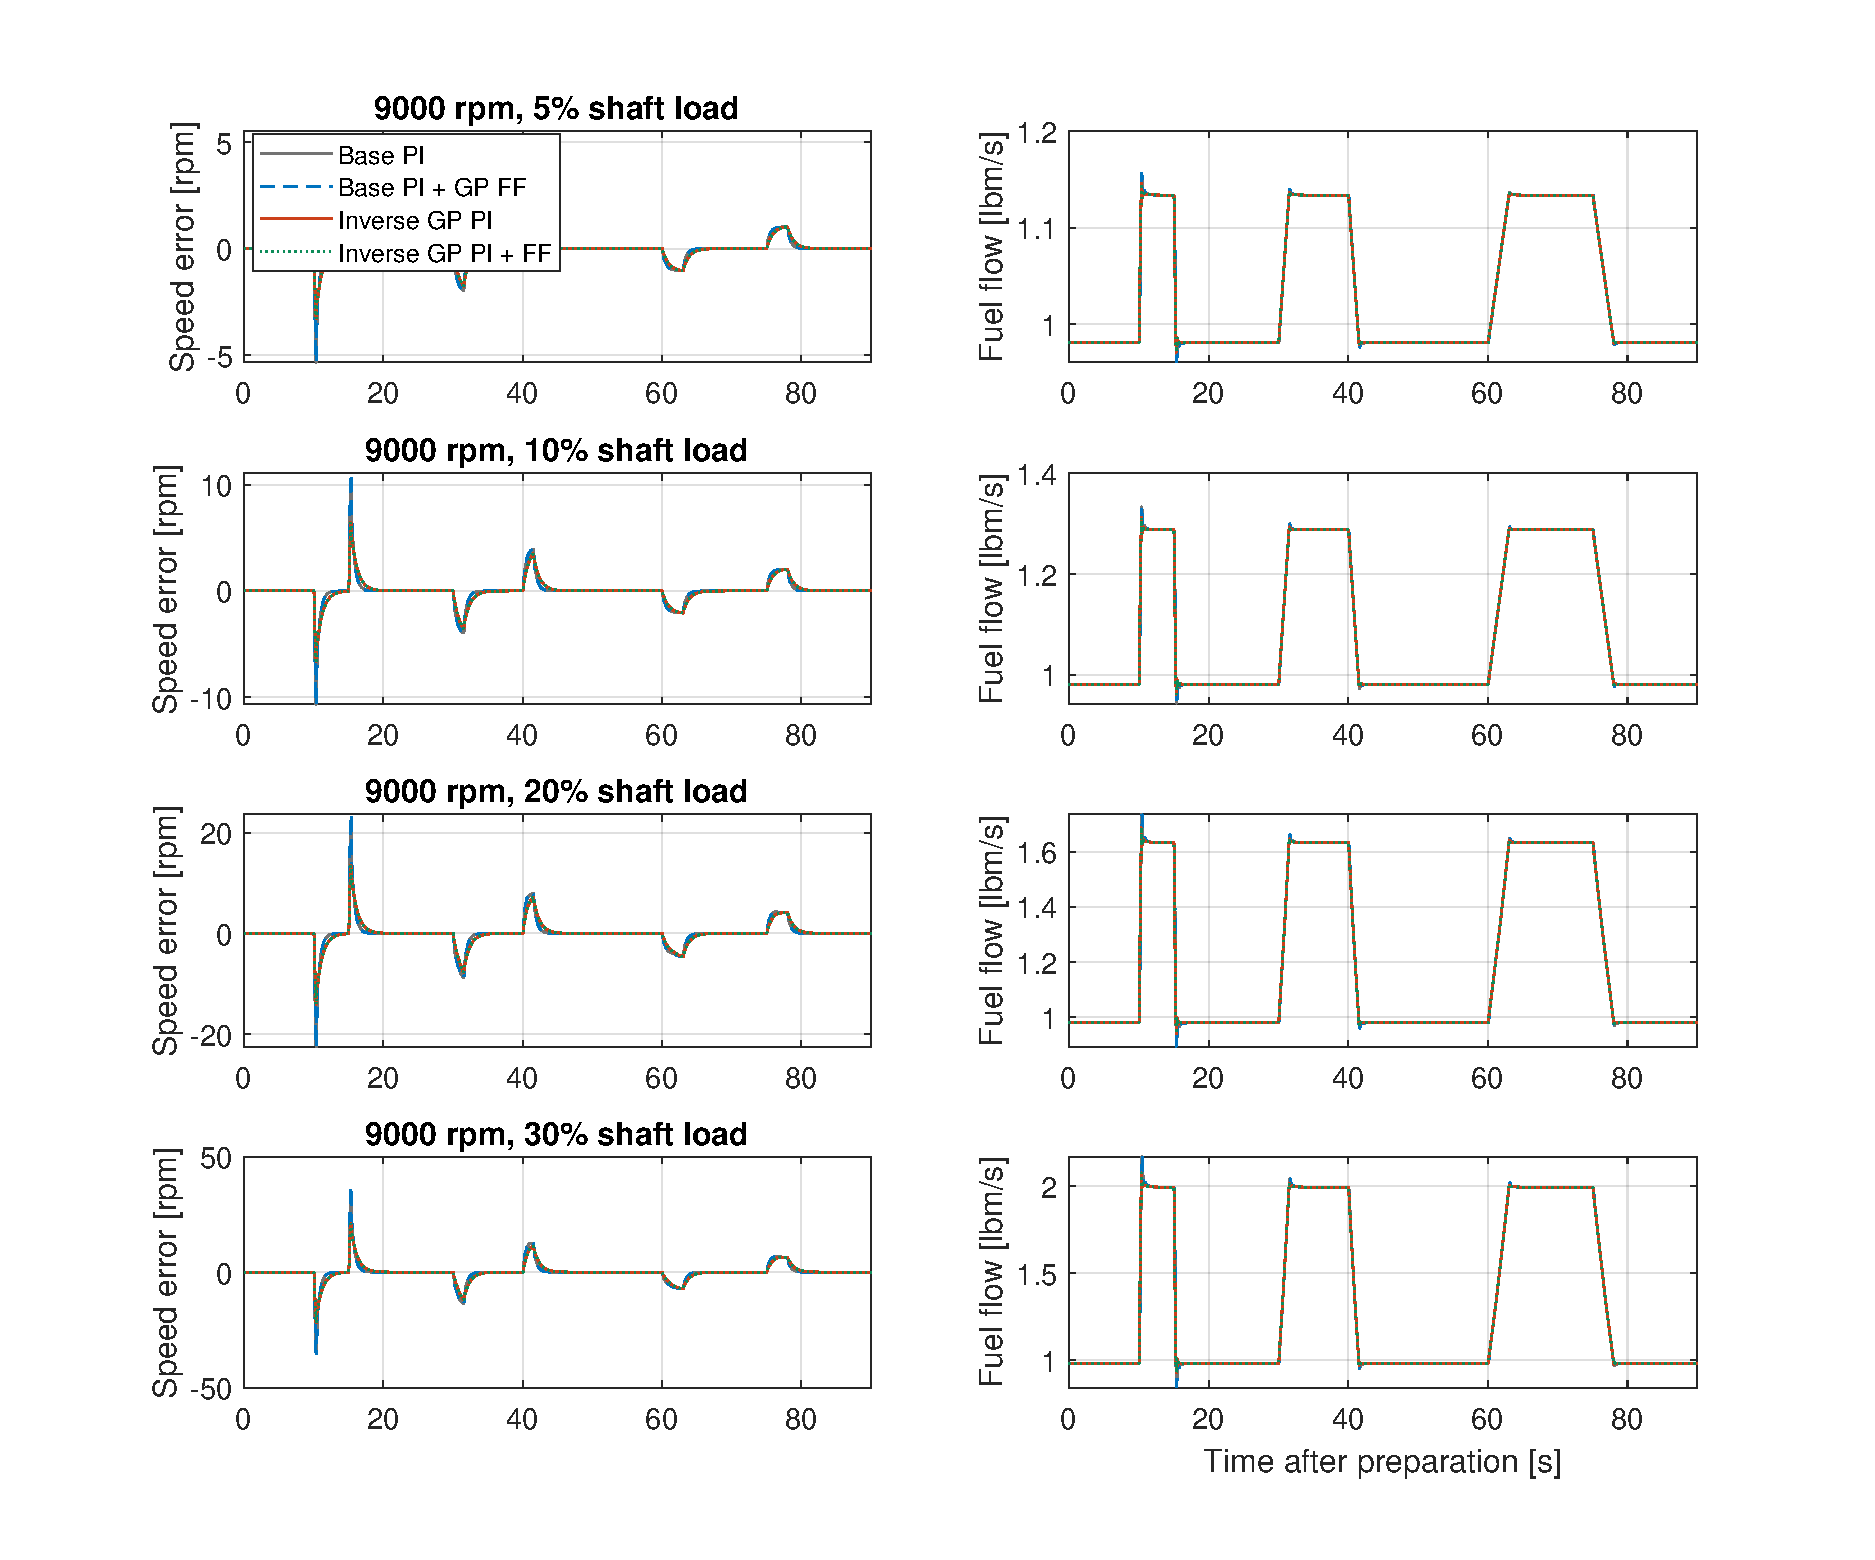
\includegraphics[width=\linewidth]{overview_9000.pdf}
\caption{Fresh 9000 rpm ramp comparisons. The inverse-GPR pair may overlap because constant feedforward is absorbed into the matched integral offset.}\end{figure}
\clearpage
\begin{figure}[H]\centering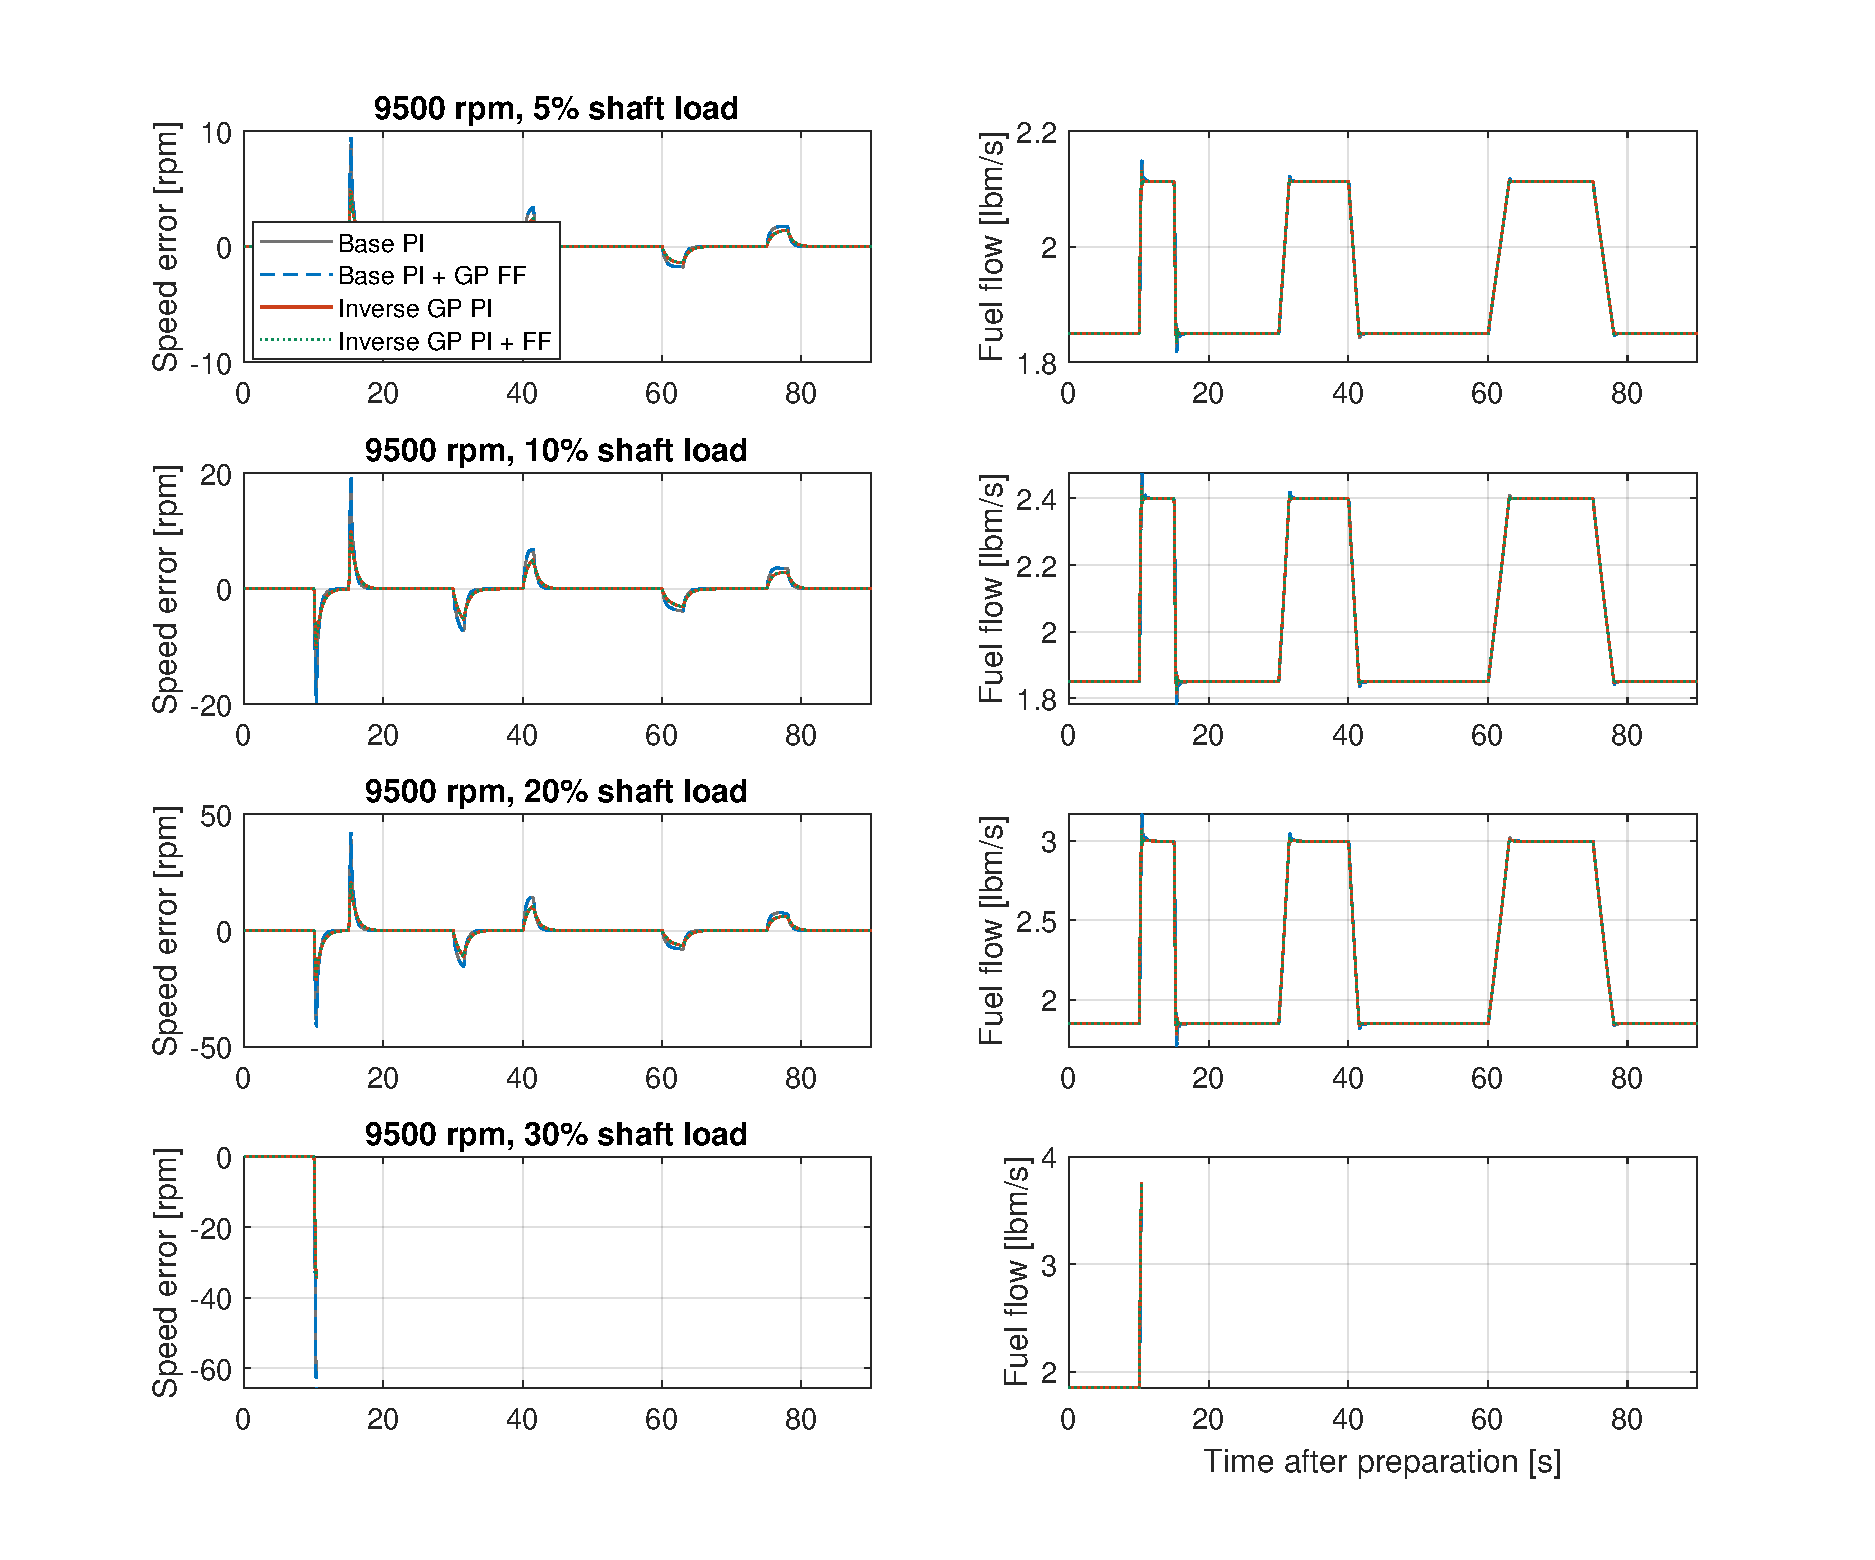
\includegraphics[width=\linewidth]{overview_9500.pdf}
\caption{Fresh 9500 rpm ramp comparisons. Traces stop at first invalid sample; high-load behavior must be interpreted with validity and minimum margin.}\end{figure}
\clearpage
\begin{figure}[H]\centering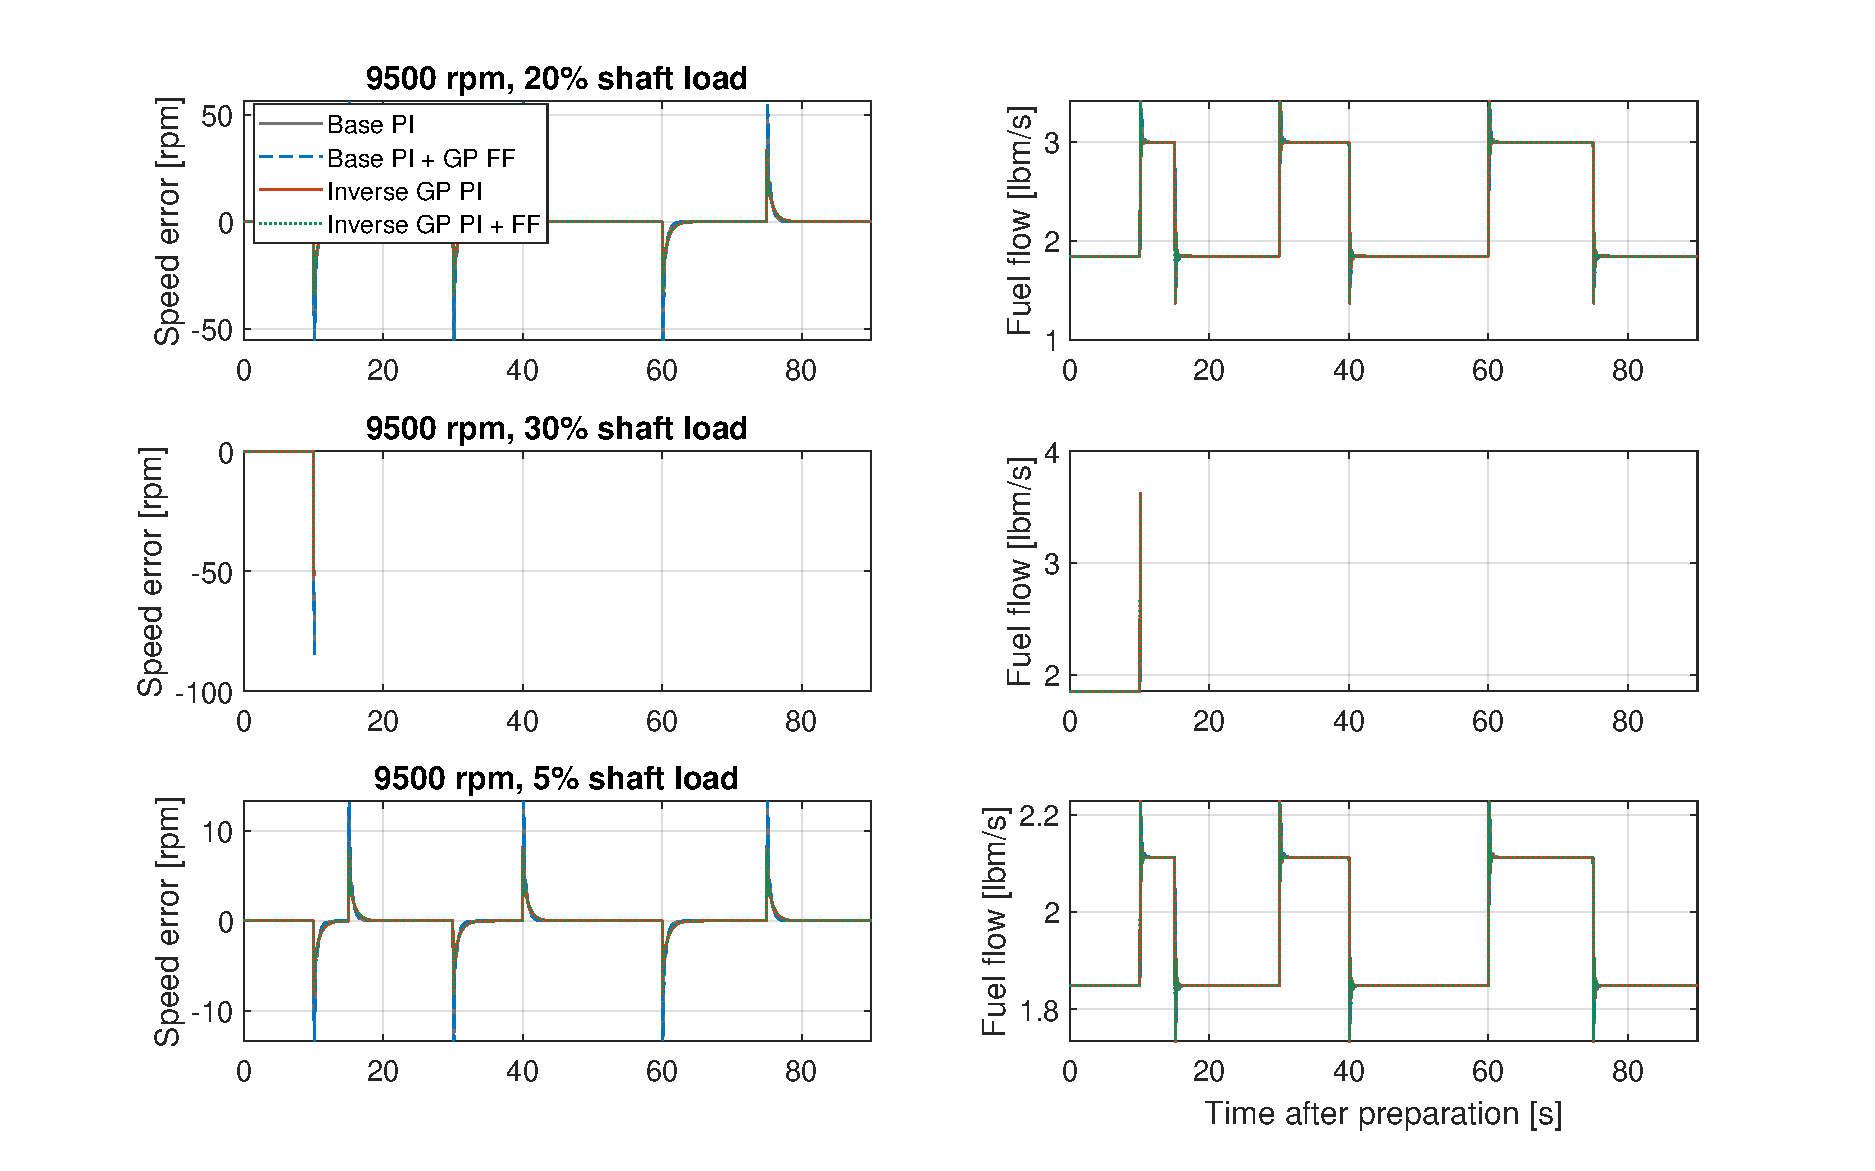
\includegraphics[width=\linewidth]{overview_steps.pdf}
\caption{Fresh 9500 rpm step comparisons: 20\%, 30\% and the 5\% tuning condition.}\end{figure}

\clearpage\subsection{Zoomed load application and removal}
\begin{figure}[H]\centering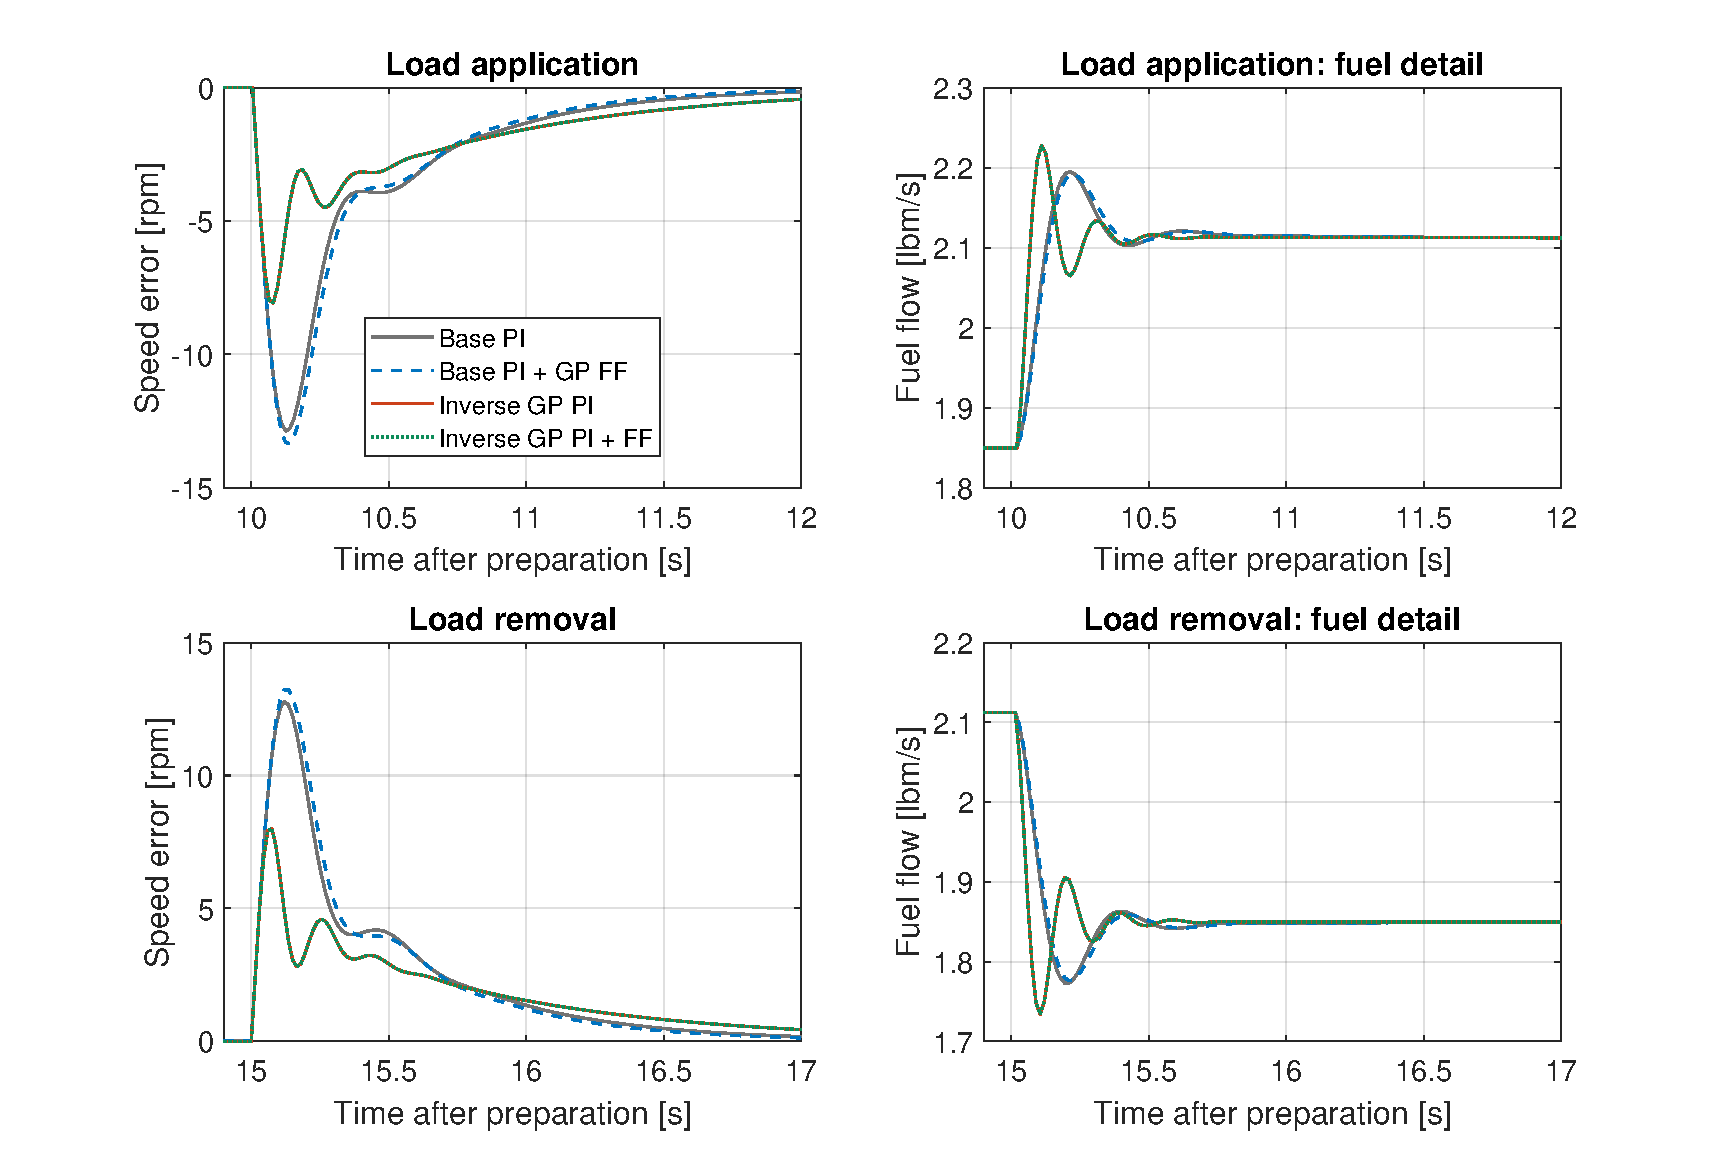
\includegraphics[width=\linewidth]{zoom_case_11.pdf}
\caption{9500 rpm, 5\% steps: speed and fuel around the first load application and removal. Short time axes expose ringing hidden in full-run plots.}\end{figure}
base PI gave RMSE 1.48 rpm, ringing 1.19 lbm/s and minimum surge margin 21\%; base PI plus GPR FF gave RMSE 1.55 rpm, ringing 1.09 lbm/s and minimum surge margin 21.1\%; inverse-GPR PI gave RMSE 0.93 rpm, ringing 2.49 lbm/s and minimum surge margin 20.6\%; inverse-GPR PI plus GPR FF gave RMSE 0.93 rpm, ringing 2.49 lbm/s and minimum surge margin 20.6\%. The retuned inverse controller still rings more than base PI on this case, despite its large reduction relative to the earlier inverse-controller gains. Its advantage here is lower speed RMSE, not minimum fuel ringing. The two-second zoom does not replace the full-event recovery measurement; it emphasizes the initial fuel reversals.
\clearpage
\begin{figure}[H]\centering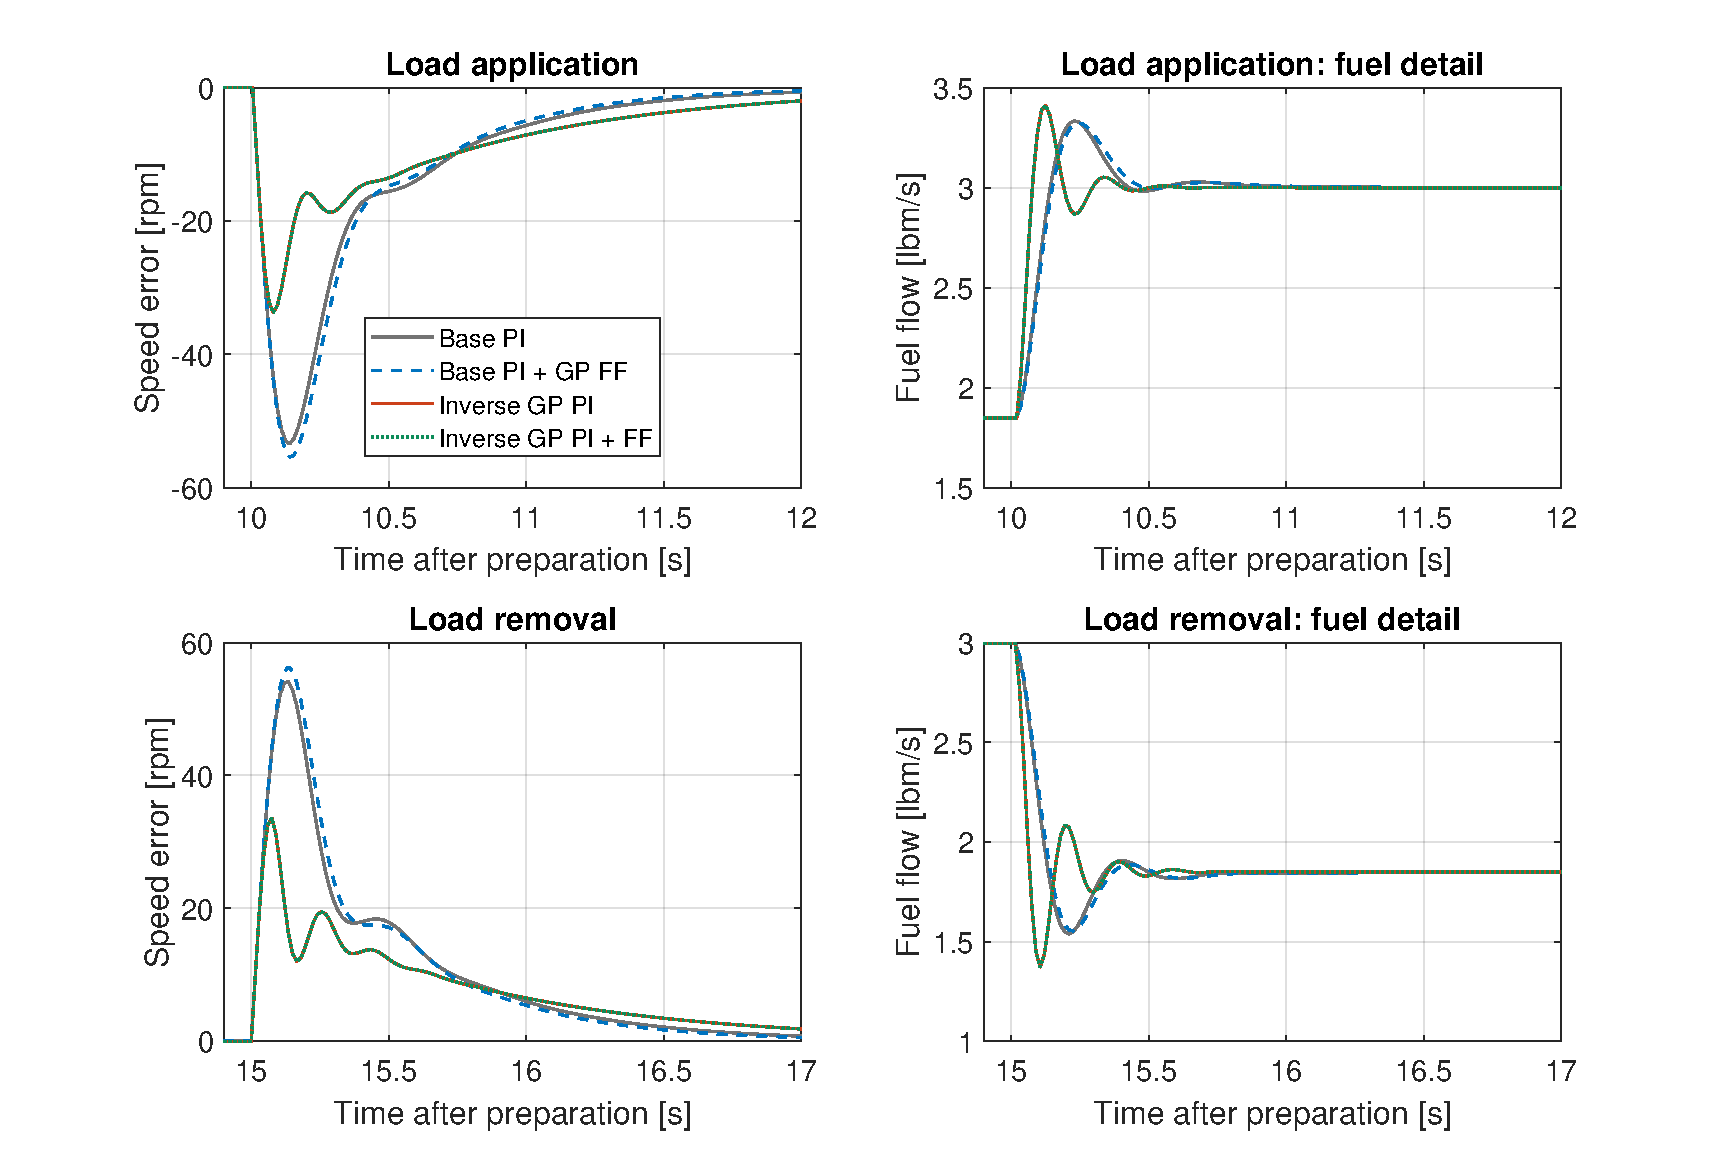
\includegraphics[width=\linewidth]{zoom_case_09.pdf}
\caption{9500 rpm, 20\% steps: transfer of the gains selected at 5\% load. A missing continuation indicates an invalid plant solve.}\end{figure}
base PI gave RMSE 6.43 rpm, ringing 4.71 lbm/s and minimum surge margin 4.86\%; base PI plus GPR FF gave RMSE 6.71 rpm, ringing 4.31 lbm/s and minimum surge margin 4.93\%; inverse-GPR PI gave RMSE 4.05 rpm, ringing 9.17 lbm/s and minimum surge margin 4.36\%; inverse-GPR PI plus GPR FF gave RMSE 4.05 rpm, ringing 9.17 lbm/s and minimum surge margin 4.36\%. This transfer result must be assessed separately from the successful 5\% tuning result.
\clearpage
\begin{figure}[H]\centering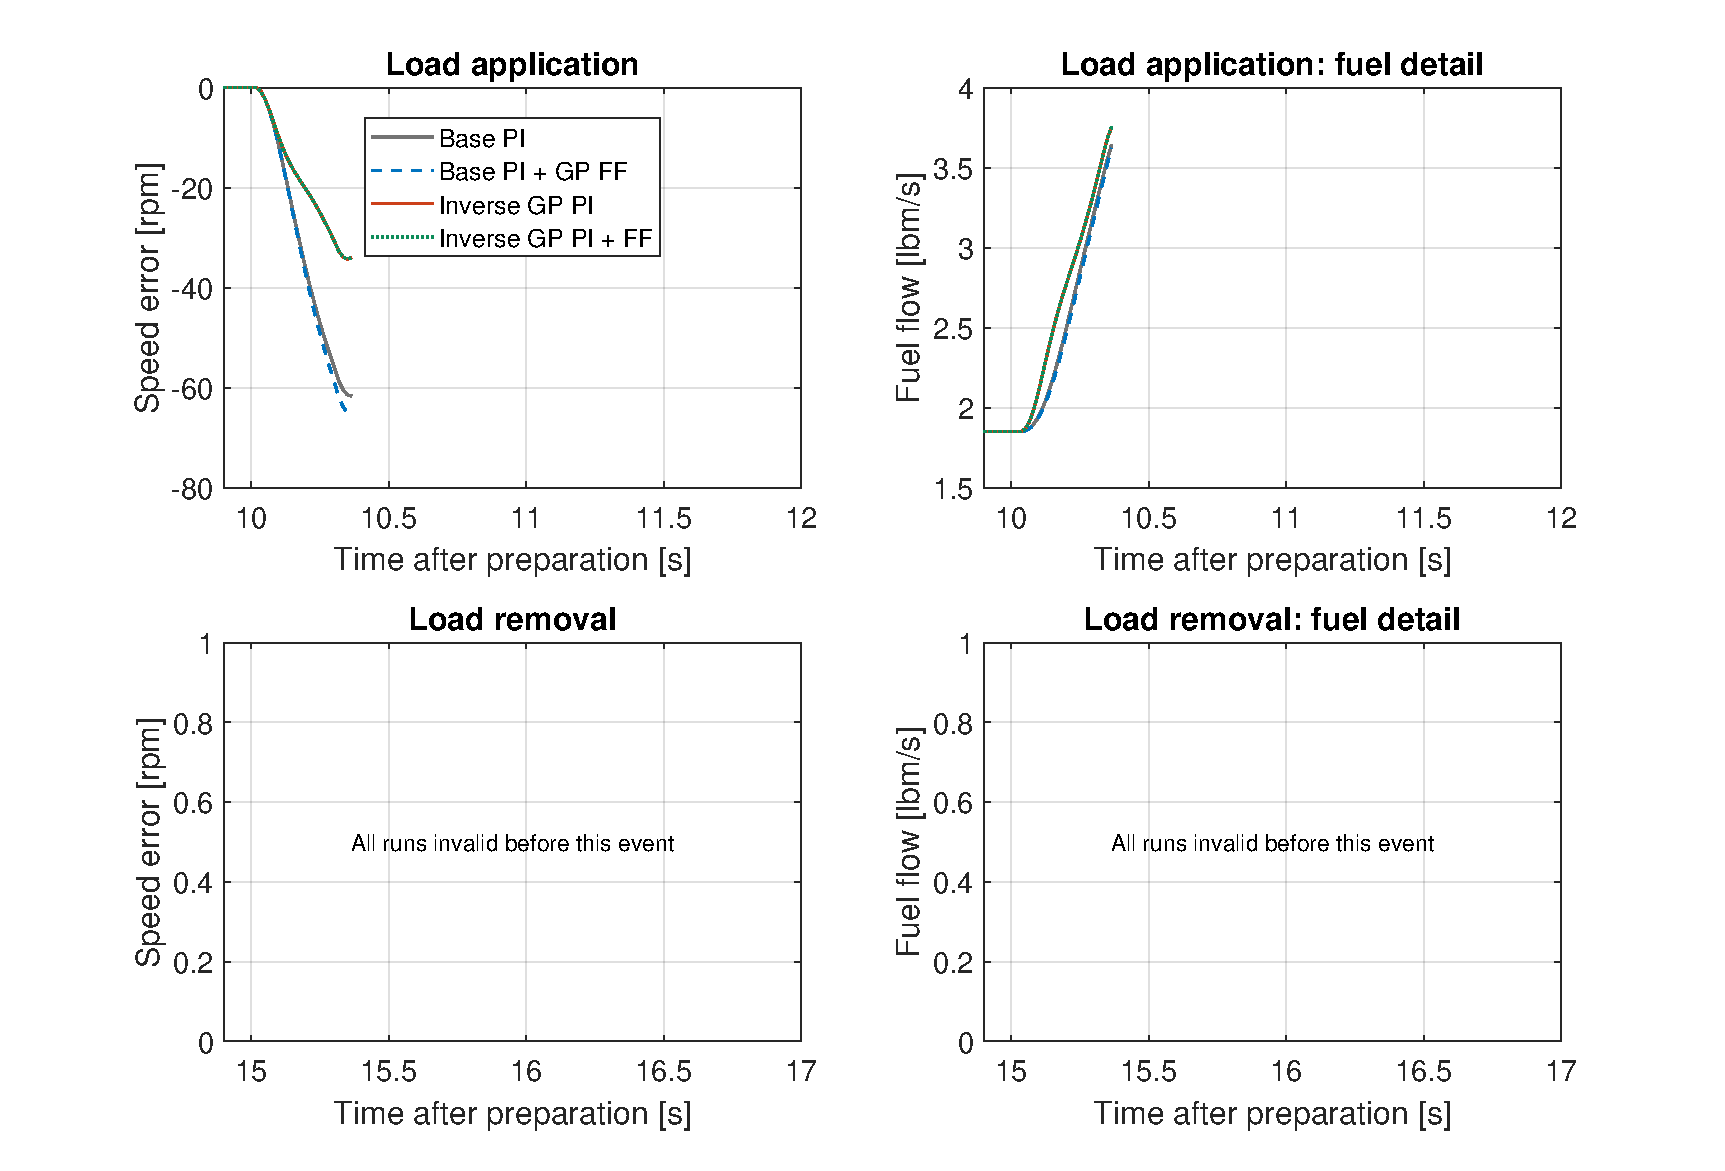
\includegraphics[width=\linewidth]{zoom_case_08.pdf}
\caption{9500 rpm, 30\% ramps: demanding load transfer. The first pulse has a 0.3 s ramp rather than an ideal step.}\end{figure}
\clearpage\subsection{Inside the selected controller}
\begin{figure}[H]\centering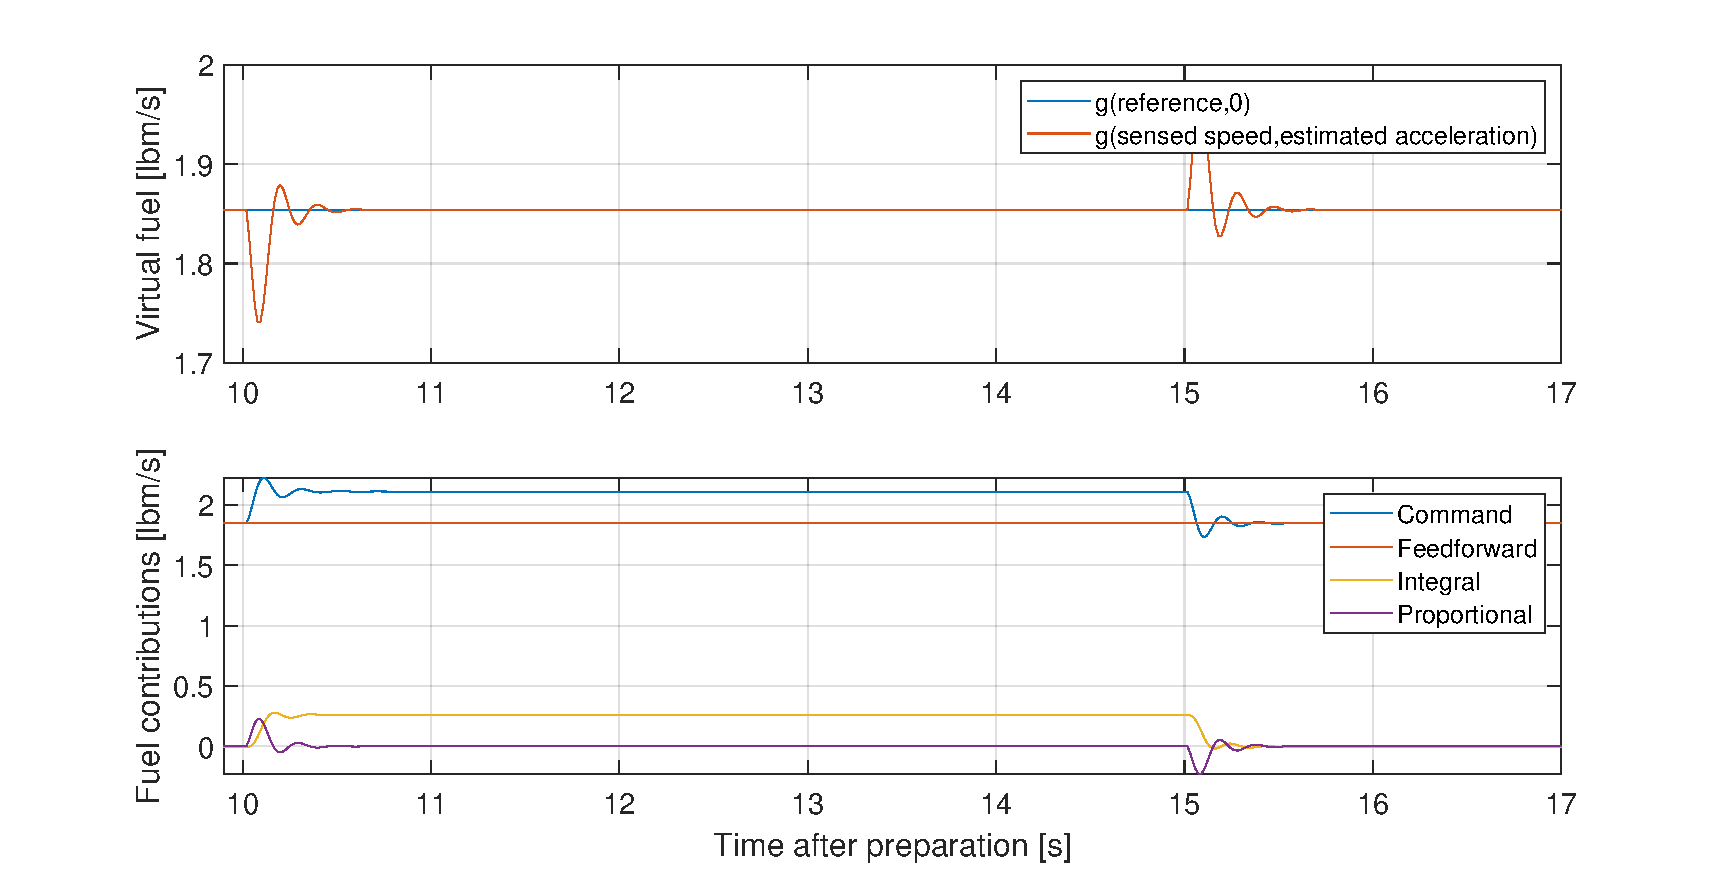
\includegraphics[width=\linewidth]{controller_components.pdf}
\caption{Virtual setpoint and feedback, then the selected FF controller's fuel contributions. The GP supplies nominal feedforward; the residual integral supports load.}\end{figure}
Over the common physically valid prefix after handover, the maximum discrepancy between the inverse-GPR pair was 2.747e-08 rpm in speed and 1.059e-09 lbm/s in fuel. These values quantify the constant-feedforward equivalence rather than presuming it from similar plots. Complete-run validity is assessed separately for each trajectory. The residual integral differs by the nominal GP feedforward offset, while the total commands match to numerical precision when the physical solves remain valid.

\section{Discussion and limits of the evidence}
The key distinction is between nominal prediction, feedback damping and disturbance accommodation. Accurate inverse prediction does not eliminate feedback tuning. A PI acting on virtual fuel contains acceleration-dependent action; treating it like an ordinary speed PI can produce unexpectedly strong fuel ringing. Lower fixed gains address that path without requiring GP uncertainty to act as a stability detector.

The selected pair is a compromise at one operating condition. The eleven-case sweep checks finite transfer conditions, not all speeds, loads, ambient conditions or sensor noise levels. A small positive surge margin is not a large operating reserve. Invalid runs are explicit and are never included in misleading average improvements.

Feedforward conclusions must follow its wiring. The base-PI correction depends on sensed speed and is bounded after equilibrium subtraction. Virtual-fuel feedforward is constant in these tests and can be absorbed into an integral offset. Overlapping inverse-GPR traces verify consistency. A changing-reference experiment would be needed to establish a separate feedforward tracking benefit.

Ringing, speed RMSE, recovery and minimum surge margin should be considered together. Lower ringing need not mean lower peak excursion or smaller speed error. The constrained tuning criterion exposes that tradeoff. The requested 1\% speed band is reported literally, with a stricter recovery column to prevent a broad-band zero from being mistaken for instantaneous physical recovery.

\section{Reproduction and data provenance}
The primary entry points are \path{run_tmats_ff_lowgain_study.m}, \path{run_tmats_four_fixed_comparison.m}, and \path{report_tmats_four_fixed_comparison.m}. The dedicated tuned model is \path{GasTurbine_Dyn_Template_LowRinging.mdl}; its setup uses 9500 rpm, 5\% steps and the selected fixed pair.

\begin{verbatim}
outTune = run_tmats_ff_lowgain_study;
out = run_tmats_four_fixed_comparison;
report_tmats_four_fixed_comparison(out);
[MWS,DOB,PTO,VF] = tmats_lowring_setup;
sim('GasTurbine_Dyn_Template_LowRinging');
\end{verbatim}
The report source package contains the complete generated \LaTeX{} document and vector figures. Compile twice with \path{pdflatex -interaction=nonstopmode Controller_Tutorial.tex}. MATLAB R2018b and the existing adjacent T-MATS library are required to rerun the plant. The exported predictor does not require refitting the GP.

Current tuning directory: \path{ff_lowgain_20260913_234549}. Final comparison directory: \path{four_fixed_20260913_235253}. Both are under the project results directory. Raw MAT/CSV files retain the signals and validity flags. Summary tables, the gain grid, selected gains, failure table and equivalence table accompany the report.

Earlier ideation evidence is archived in \path{inverse_gpr_20260913_150824_698}, \path{virtual_fuel_20260913_182229_028}, \path{virtual_fuel_ff_20260913_194955}, \path{virtual_fuel_uq_20260913_201212}, and \path{virtual_fuel_uqup_20260913_231743}. Controller equations and local interpretations are derived for this project; the references support the nominal GP formulation and T-MATS plant framework, not a claimed closed-loop theorem.
\begin{thebibliography}{9}
\bibitem{gpml} C. E. Rasmussen and C. K. I. Williams, \emph{Gaussian Processes for Machine Learning}, MIT Press, 2006, Chapter 2. \url{https://gaussianprocess.org/gpml/chapters/RW2.pdf}.
\bibitem{tmats} J. W. Chapman, T. M. Lavelle, R. D. May, J. S. Litt and T.-H. Guo, \emph{Toolbox for the Modeling and Analysis of Thermodynamic Systems (T-MATS) User's Guide}, NASA/TM-2014-216638, 2014. \url{https://ntrs.nasa.gov/archive/nasa/casi.ntrs.nasa.gov/20140012486.pdf}.
\end{thebibliography}
\end{document}
